\section{Hardware}
Das Endprodukt setzt sich hauptsächlich aus dem Melde- und Sensor-Print zusammen. In den nachfolgenden Kapiteln werden alle Teilschaltungen beschrieben um einen möglichen Nachbau zu erleichtern.
\subsection{Sensorprint}
Das folgende Kapitel beschreibt den Hardwareaufbau des Sensorprints zuerst grob, danach wird die Schaltung weiter unterteilt und jeder Bereich einzeln erläutert.

Jedes Solarpannel wird mit einem Sensorprint auf der Rückseite des Pannels bestückt. Der Aufbau des Sensorprints besteht aus einem Mikrocontroller, einem Powerline Transceiver, einem ADC Converter und einer 12V Speisung. Seine Aufgabe ist die Spannungswerte des Solarpannels einzulesen, diese zu verarbeiten und die Informationen über die Powerline an den Meldeprint zu übermitteln. Eine grobe Übersicht über den Aufbau und das zusammenspielen der einzelnen Komponenten gibt die nachfolgende Abbildung.

Abbildung..


\subsubsection{Speisung}
Die Speisung des Sensorprints erfolgt über einen LM 2594 DC/DC Regulator. Dieser erhält eine variable Eingangsspannung von 12V - 60V vom Solarpannel. Der DC/DC Regulator regelt diese Eingangsspannung mit hilfe eines Schaltreglers auf eine feste 12V DC Spannung am Ausgang. Diese Spannung gewährleistet die Versorgung des Powerline Transceivers. Die restlichen Elemente werden mit 5V gespiesen.

Die 5V DC Spannung wurde anders als geplannt realisiert. Auf dem Print war nur Platz für eine Speiseschaltung vorgesehen, darum musste die 5V Spannung über den 5V Ausgang des Powerline Transceivers realisiert werden. Da nur eine sehr geringe Leistungen auf dem Sensorprint vorhanden ist, ist diese Beschaltung vertretbar.

In der nachfolgenden Abbildung ist die Beschaltung der 12V Speisung ersichtlich.

Abildung..

\subsubsection{Spannungsmessung}
Die Spannungsmessung erfolgt über einen Analog - Digital - Converter (MCP 3202). Am Analog Input (Ch0) des ADC's wird die Spannung des Solarpannels eigelesen. Da nur 0V - 5V eingelesen werden können wird die Spannung mit einem Spannungsteiler entsprechend skaliert. Der Analoge Wert wird vom ADC in einen binären 12 Bit Wert (0V = 0000 0000 0000, 5V = 1111 1111 1111) umgewandelt und über den Digitalen Output (Dout) zum Mikrocontroller übertragen. Ein 12 Bit ADC wurde gewählt, um die Genauigkeit der Spannungsmessung von 0.1V zwischen 12V und 60V zu gewährleisten.

Um den Ablauf der Umwandlung besser nachvollziehen zu können, ist in der nachfolgenden Abbildung ist die innere Architektur des Analog - Digital - Converters ersichtlich.

Abbildung..

\subsubsection{Mikrocontroller}
Als zentrale Steuereinheit des Sensorprints haben wir einen Arduino Nano Board mit einem Atmega 328 Chip ausgewählt. Dieses Board wurde gewählt, weil vereinzelte Vorkenntnisse bereits vorhanden waren. Als Verbesserung könnte man den Atmega 328 und seine Grundbeschaltung direkt auf den Print bestücken. Somit könnte man mehr Platz sparen und den Print noch komprimierter herstellen.

Die Aufgabe des Mikrocontrollers auf dem Sensorprint beruht im allgemeinen darauf, die Verbindung zwischen dem ADC und dem Powerline Transceiver herzustellen. Die Verbindung zwischen Mikrocontroller und ADC wird mit SPI Kommunikation hergestellt. Die Verbindung zum Powerline Transceiver wird über UART Kommunikation hergestellt. Detailiertere Informationen zur Kommunikation der einzelnen Elemente untereinander sind im Abschnitt 4.1 unter Software vorhanden.

\subsubsection{Adressierung}
Um das Pannel identifizeren zu können, wurde Hardware basierend eine binäre Adressierung hergestellt. Diese erfolgt über einen binären 8 Bit Wert, welcher mit Dip - Switch Schaltern eingestellt werden kann. Dieser wird parallel an 8 Eingängen am Mikrocontroller eingelesen. Mit 8 Schaltern können somit 256 Pannels adressiert werden. Die Beschaltung der Schalter ist in der nachfolgenden Abbildung ersichtlich.

Abbildung..

\subsubsection{Transceiver}
\subsubsection{Layout}

\subsection{Meldeprint}
%Der Hardwareaufbau des Meldeprints wird in diesem Kapitel zuerst grob beschrieben, anschliessend wird die Schaltung weiter aufgeteilt und jeder Bereich einzeln erläutert.
Der Meldeprint hat zur Aufgabe die von den einzelnen Panels übertragenen Informationen zu empfangen und diese auszuwerten. Er entscheidet, ob ein Panel fehlerhaft ist und zeigt dieses auf einem Display an. Der Meldeprint ist grundlegend aufgeteilt in die folgenden Schaltungsteile: Speisung, Mikrocontroller, Powerline Transceiver sowie Bedienung und Ausgabe.

\begin{figure}[h]
	\centering
	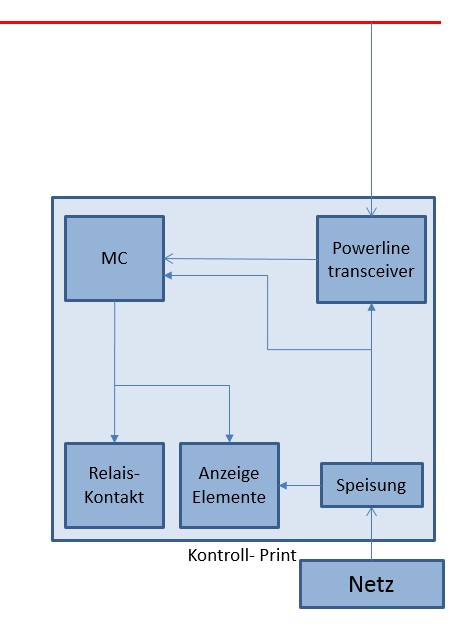
\includegraphics[width=0.5\textwidth]{konzept_melde.PNG}
	\caption{Grobkonzept des Meldeprints}	
\end{figure}

\subsubsection{Speisung}
Als Speisung wird ein 230V-AC/DC Netzgerät genommen. Dieses wandelt die Spannung in 24V DC um welche wiederum mit zwei weiteren DC/DC Wandlern in 12V für die Speisung des Mikrocontrollers und des Powerline Transceivers respektive 5V für die Logik Schaltung. Das 24V-AC/DC Netzteil wurde gewählt da diese Spannung im Eingangsspannungsbereich der meisten DC/DC-Wandler liegt und so eine erhöhte Flexibilität in der Wahl dieser erlaubt. Für die DC/DC-Wandler wurden 2 Traco Power Step-Down Converter gewählt weil diese keine externe Beschaltung benötigen und einen Wirkungsgrad grösser als 90 Prozent haben.

\subsubsection{Mikrocontroller}
Es wurde ein Arduino UNO als Mikrocontroller eingesetzt. Der UNO wurde gewählt, da dieser die benötigte Anzahl Ports besitzt, über einen genügend grossen Speicherplatz verfügt. Ein weiterer Vorteil waren die bereits angesammelten Fachkenntnisse in der Bedienung durch das Modul mc1, welche den Aufbau erleichterten.

Der Mikrocontroller regelt das empfangen der Informationen der einzelnen Solarpanels sowie das Auswerten von diesen inbegrifflich der Erkennung von Übertragugnsfehlern. Er hat die Aufgabe die empfangenen Daten in einer sinnvollen Struktur abzulegen und den Mittelwert sowie die Standardabweichung von den Spannungswerten bilden zu können. Eine Spannungsabweichung eines Solarpanels soll zu einer Fehlermeldung führen, die anhand einer LED zu erkennen ist, sowie der Anzeige der ID des fehlerhaften Moduls am Display. Desweiteren wird ein Relaiskontakt geschlossen, an welchen man mittels herkömmlichen Laborbuchsen ein externes Gerät anschliessen kann.

Der Mikrocontroller liest den Status des Inkrementalgebers ein, welcher für die Menüführung zuständig ist. Der Mikrocontroller kann mittels eines Reset Tasters in den Originalzustand zurückversetzt werden, welches alle momentane Messwerte löscht.

\subsubsection{Receiver}
Als Powerline Transceive wurde wie schon beim Sensor-Print der ST7540 genommen. Die Beschaltung entspricht derjenigen vom Sensor-Print, als Design Grundlage für die Filterschaltung wurde der Application Guide \cite[p. 48]{Applic_Guide_ST7540} von STMicroelectrinics verwendet. Als Übertragungsfrequenz wurde 132.5kHz gewählt. Für die Grundbeschaltung wurde das Datenblatt des ST7540 \cite[p. 40]{Datasheet_ST7540} als Referenz genommen. Die Einkopplung der Powerline ist wiederum induktiv, sie wird mit einem Ferrit Kern verwirklicht um den ein isolierter Draht gewickelt wurde (Spule).
Es wurde anfangs des Projektes gegen die Entwicklung einer eigenen Powerline-Communication entschieden aufgrund des grossen Zeitaufwandes sowohl für die Erarbeitung der Theorie für die Frequenzmodulation, als auch der Entwicklung selbst. Stattdessen wurde zugunsten eines Integrierten Bausteins entschieden. Der ST7540 wurde gewählt, da 8 Übertragungsfrequenzen bereits vorprogrammiert sind sowie auch 4 Baudraten. Für die Dimensionierung der Beschaltung waren das Datenblatt \cite{Datasheet_ST7540} sowie ein Application Guide \cite{Applic_Guide_ST7540} verfügbar, dies vereinfachte die Auswahl der Bauteile für die Filterschaltungen (siehe Kapitel \ref{sec::Theorie}).

%\subsubsection{Layout}
\subsubsection{Bedienung und Ausgabe}
Zur Bedienung des Gerätes dient ein Inkrementalgeber, mit welchem man sich durch das Menü des Displays navigieren kann. Die Ausgabe der Messwerte sowie der Fehlermeldungen geschieht auf dem Display. Bei einer Fehlermeldung leuchtet zusätzlich noch eine LED an der Front des Gehäuses und ein Relaiskontakt wird geschlossen. An diesen Kontakt kann mittels zwei Laborbuchsen ein externes Gerät angeschlossen werden. Das verwendete Relais ist das Siemens V23026 \cite{Siemens_Rel}, welches eine Nennspannung von 5V hat und einen Schaltstrom von maximal 1A hat. Des weiteren kann eine Last von bis zu 30W getrieben werden, was den Vorteil hat, das externe Geräte angeschlossen werden können und das Relais direkt mit dem Mikrocontroller geschaltet werden kann.

%\subsubsection{(Gehäuse)}
